% -*- mode:LaTeX; mode:flyspell; -*-
\documentclass{article}

% Almost always
\usepackage{enumerate}
\usepackage{booktabs}
\usepackage{amsmath, amsthm}
\usepackage{graphicx}
\usepackage{hyperref}
\usepackage[verbose,letterpaper,top=1.25in,bottom=1in,left=1.25in,right=1.25in]{geometry}

\setlength{\parindent}{0pt}
\setlength{\parskip}{\baselineskip}


% extra stuff for assignments
\newcounter{totalpoints}
\setcounter{totalpoints}{0}

\newcommand{\points}[1]{{\addtocounter{totalpoints}{#1}\textbf{[#1 points]}}}
\usepackage{environ}
\usepackage{etoolbox}
\makeatletter
\NewEnviron{answer}[1]
{\ifx\BODY\@empty
 \vspace{#1}%
\else
 {\sf \BODY}%
\fi}
\makeatother

\usepackage{totcount}
\regtotcounter{totalpoints}
\begin{document}

{\bigskip\hrule\bigskip
\huge
\noindent CMPUT 366, Winter 2022\\
Assignment \#4

\large
Due: Friday, April 15, 2022, 11:59pm\\
Total points: \total{totalpoints}

For this assignment use the following consultation model:
\begin{enumerate}

\item you can discuss assignment questions and exchange ideas with other \emph{current} CMPUT~366 students;

\item you must list all members of the discussion in your solution;

\item you may {\bf not} share/exchange/discuss written material and/or code;

\item you must write up your solutions individually;

\item you must fully understand and be able to explain your solution in any amount of detail as requested by the instructor and/or the TAs.

\end{enumerate}

Anything that you use in your work and that is not your own creation must be properly cited by listing the original source. Failing to cite others' work is plagiarism and will be dealt with as an academic offence.

%%%%%%%%%%%%%%%%%%%%%%%%%%%%%%%%%%%%%

\bigskip\bigskip\hrule\bigskip

\vspace{1cm}
\hspace{1cm}{\bf First name:} \underline{\hspace{7cm}}

\vspace{1cm}
\hspace{1cm}{\bf Last name:} \underline{\hspace{7cm}}

\vspace{1cm}
\hspace{1cm}{\bf CCID:} \underline{\hspace{5.5cm}}\verb|@ualberta.ca|

\vspace{1cm}
\hspace{1cm}{\bf Collaborators:} \underline{\hspace{6.5cm}}

\vspace{1cm}
\bigskip\hrule\bigskip
}

\pagestyle{myheadings}
\markboth{}{CMPUT 366 --- Assignment \#4}

\begin{enumerate}

%------------------------------------------------------------------------------------------
\item \textbf{(Markov Decision Processes)}

    Two coins are placed in a tray; each coin is either heads up or tails up with equal probability, independent of the other coin.  A robot arm is above \textbf{one} of the coins.  At each time step, the arm can perform one of the following operations:
    \begin{itemize}
        \item \texttt{Flip} the coin that it is above: The coin under the arm will be randomly set to either heads up or tails up with equal probability.  This operation costs 1 unit of battery power.
        \item \texttt{Move} to be above the other coin; this operation costs 2 units of battery power.
        \item \texttt{Call} the Electricity Fairy, who will reward the robot with 20 units of battery power if both coins are heads up, reward the robot with 10 units of battery power if both tails are up, or fine the robot 5 units of electricity if the coins mismatch.  After rewarding or fining the robot, the Electricity Fairy will then flip both coins before leaving.
    \end{itemize}
\begin{enumerate}
    \item\points{10}
    Represent this scenario formally as a Markov Decision Process, treating changes in battery power as the reward signal.

    \textbf{Note:} You do not need to include the total battery charge as part of the state.  Changes in battery charge are reward only.  (I.e., the battery never runs out; its charge can become negative and the robot can keep operating.)
    
    \begin{answer}{2.5in}
    % Put your answer here
    \end{answer}

    \item\points{2}
    Is this a continuing or episodic scenario?  Justify your answer.
    \begin{answer}{.75in}
    % Put your answer here
    \end{answer}

    \item\points{3}
    If you answered episodic to the previous question, describe how to treat the scenario as continuing.
    If you answered continuing to the previous question, describe how to treat the scenario as episodic.
    \begin{answer}{1in}
    % Put your answer here
    \end{answer}
\end{enumerate}


%------------------------------------------------------------------------------------------
\item \textbf{(Bellman Action-Value Equation)}
\begin{enumerate}
    \item\points{4}
    Give an expression for $q_\pi(s,a)$ as an expectation of random variables, in the same form as equation (4.3) in the text.
    \begin{answer}{.5in}
    % Put your answer here
    \end{answer}

    \item\points{4}
    Give an expression for $q_\pi(s,a)$ as a weighted sum, in the same form as equation (4.4) in the text.
    \begin{answer}{.5in}
    % Put your answer here
    \end{answer}
\end{enumerate}

%------------------------------------------------------------------------------------------
\item \textbf{(Policy Improvement)}
Consider the following MDP with actions $\mathcal{A}=\{a,b\}$, states $\mathcal{S}=\{W,X,Y,Z\}$, and the following dynamics.  All unspecified transitions have probability 0:

\begin{align*}
    p(X,4|W,a) &=0.5  & p(Z,0|X,a) &= 0.8    &  p(Z,1|Y,a) &=1 \\
    p(Y,2|W,a) &=0.5  & p(Z,25|X,a) &=0.2   &  p(Z,5|Y,b) &=1 \\
    p(Z,3|W,b) &= 1   & p(Z,0|X,b) &= 1      &  p(Z,0|Z,a) &=1 \\
               &      &            &         &  p(Z,0|Z,b) &=1\\
\end{align*}

\begin{enumerate}
    \item\points{4}
    Consider the policy $\pi(b|s) = .5, \pi(a|s)=.5$ for all states $s\in\mathcal{S}$; i.e., a policy that randomizes between the two actions uniformly.
    Using a discount rate of $\gamma=0.8$, what is the value $v_\pi(s)$ for each state $s\in\mathcal{S}$?
    (Hint: What must the value of state $Z$ be under any policy?)
    \begin{answer}{1.5in}
    % Put your answer here
    \end{answer}

    \item\points{8}
    Construct a policy $\pi'$ that strictly improves upon $\pi$: That is, $v_{\pi'}(s) \ge v_\pi(s)$ for all $s\in\mathcal{S}$, and $v_{\pi'}(s) > v_\pi(s)$ for at least one $s \in \mathcal{S}$.  Appeal to the Policy Improvement Theorem to show that your new policy is indeed a strict improvement.
    \begin{answer}{1.5in}
    % Put your answer here
    \end{answer}
\end{enumerate}

\item \textbf{(Monte Carlo Prediction)}
Consider an MDP with actions $\mathcal{A}=\{a,b,c\}$, states $\mathcal{S}=\{W,X,Y,Z\}$ (with terminal state $Z$), and unknown dynamics.
Suppose that you have used a policy $\pi$ to generate 4 episodes with the following trajectories:
\begin{align*}
    &\langle S_0=W, A_0=a, R_1=0, S_1=X, A_1=a, R_2=10, S_2=Y, A_2=b, R_3=0, S_3=Z\rangle,\\
    &\langle S_0=W, A_0=a, R_1=-10, S_1=X, A_1=b, R_2=0, S_2=Z\rangle,\\
    &\langle S_0=W, A_0=b, R_1=2, S_1=Y, A_1=c, R_2=6, S_2=Z\rangle,\\
    &\langle S_0=W, A_0=b, R_1=0, S_1=Y, A_1=c, R_2=12, S_2=Z\rangle.
\end{align*}
\begin{enumerate}
    \item \points{8}
    Use first-visit Monte Carlo prediction to estimate $v_\pi(s)$ for every $s\in\mathcal{S}$.  Assume undiscounted rewards (i.e., $\gamma=1$).

    \begin{answer}{1.5in}
    % Put your answer here
    \end{answer}
\end{enumerate}

%------------------------------------------------------------------------------------------
\item \textbf{(Temporal Difference Control)}
Consider an MDP with actions $\mathcal{A}=\{a,b,c\}$, states $\mathcal{S}=\{W,X,Y\}$, and unknown dynamics.

Suppose that you have previously computed the following estimated action values:
\begin{align*}
    Q(W,a) &= 0  &  Q(X,a) &= 8   &      Q(Y,a) &= 0  \\
    Q(W,b) &= 0  &  Q(X,b) &= 7   &      Q(Y,b) &= 0  \\
    Q(W,c) &= 0  &  Q(X,c) &= 16  &      Q(Y,c) &= 0  \\
\end{align*}

Now suppose that starting from state $S_t=W$, the current behaviour policy selects action $A_{t}=a$, leading to reward $R_{t+1}=4$ and a transition to state $S_{t+1}=X$.  The behaviour policy then selects action $A_{t+1}=a$.

\begin{enumerate}
    \item \points{6}
    What is the updated estimate for $Q(W,a)$ according to the $Q$-learning algorithm?
    Assume a step size of $\alpha=0.5$ and a discount rate of $\gamma=1$.
    \begin{answer}{1.5in}
    % Put your answer here
    \end{answer}

    \item \points{6}
    What is the updated estimate for $Q(W,a)$ according to the Sarsa algorithm?
    Assume a step size of $\alpha=0.5$ and a discount rate of $\gamma=1$.
    \begin{answer}{1.5in}
    % Put your answer here
    \end{answer}

\end{enumerate}


%------------------------------------------------------------------------------------------
\newpage
\item \textbf{(Programming)} \points{40}
Consider the following task (pictured in Figure~\ref{fig:q6}): an intrepid adventurer must make his way through a maze. To do so, he must first collected a key, located somewhere in the maze, before leaving through a door. Without the key, the door will not open. Additionally, the maze contains dangerous fire hazards, which the adventurer wishes to avoid.  

 \begin{figure}
    \centering
    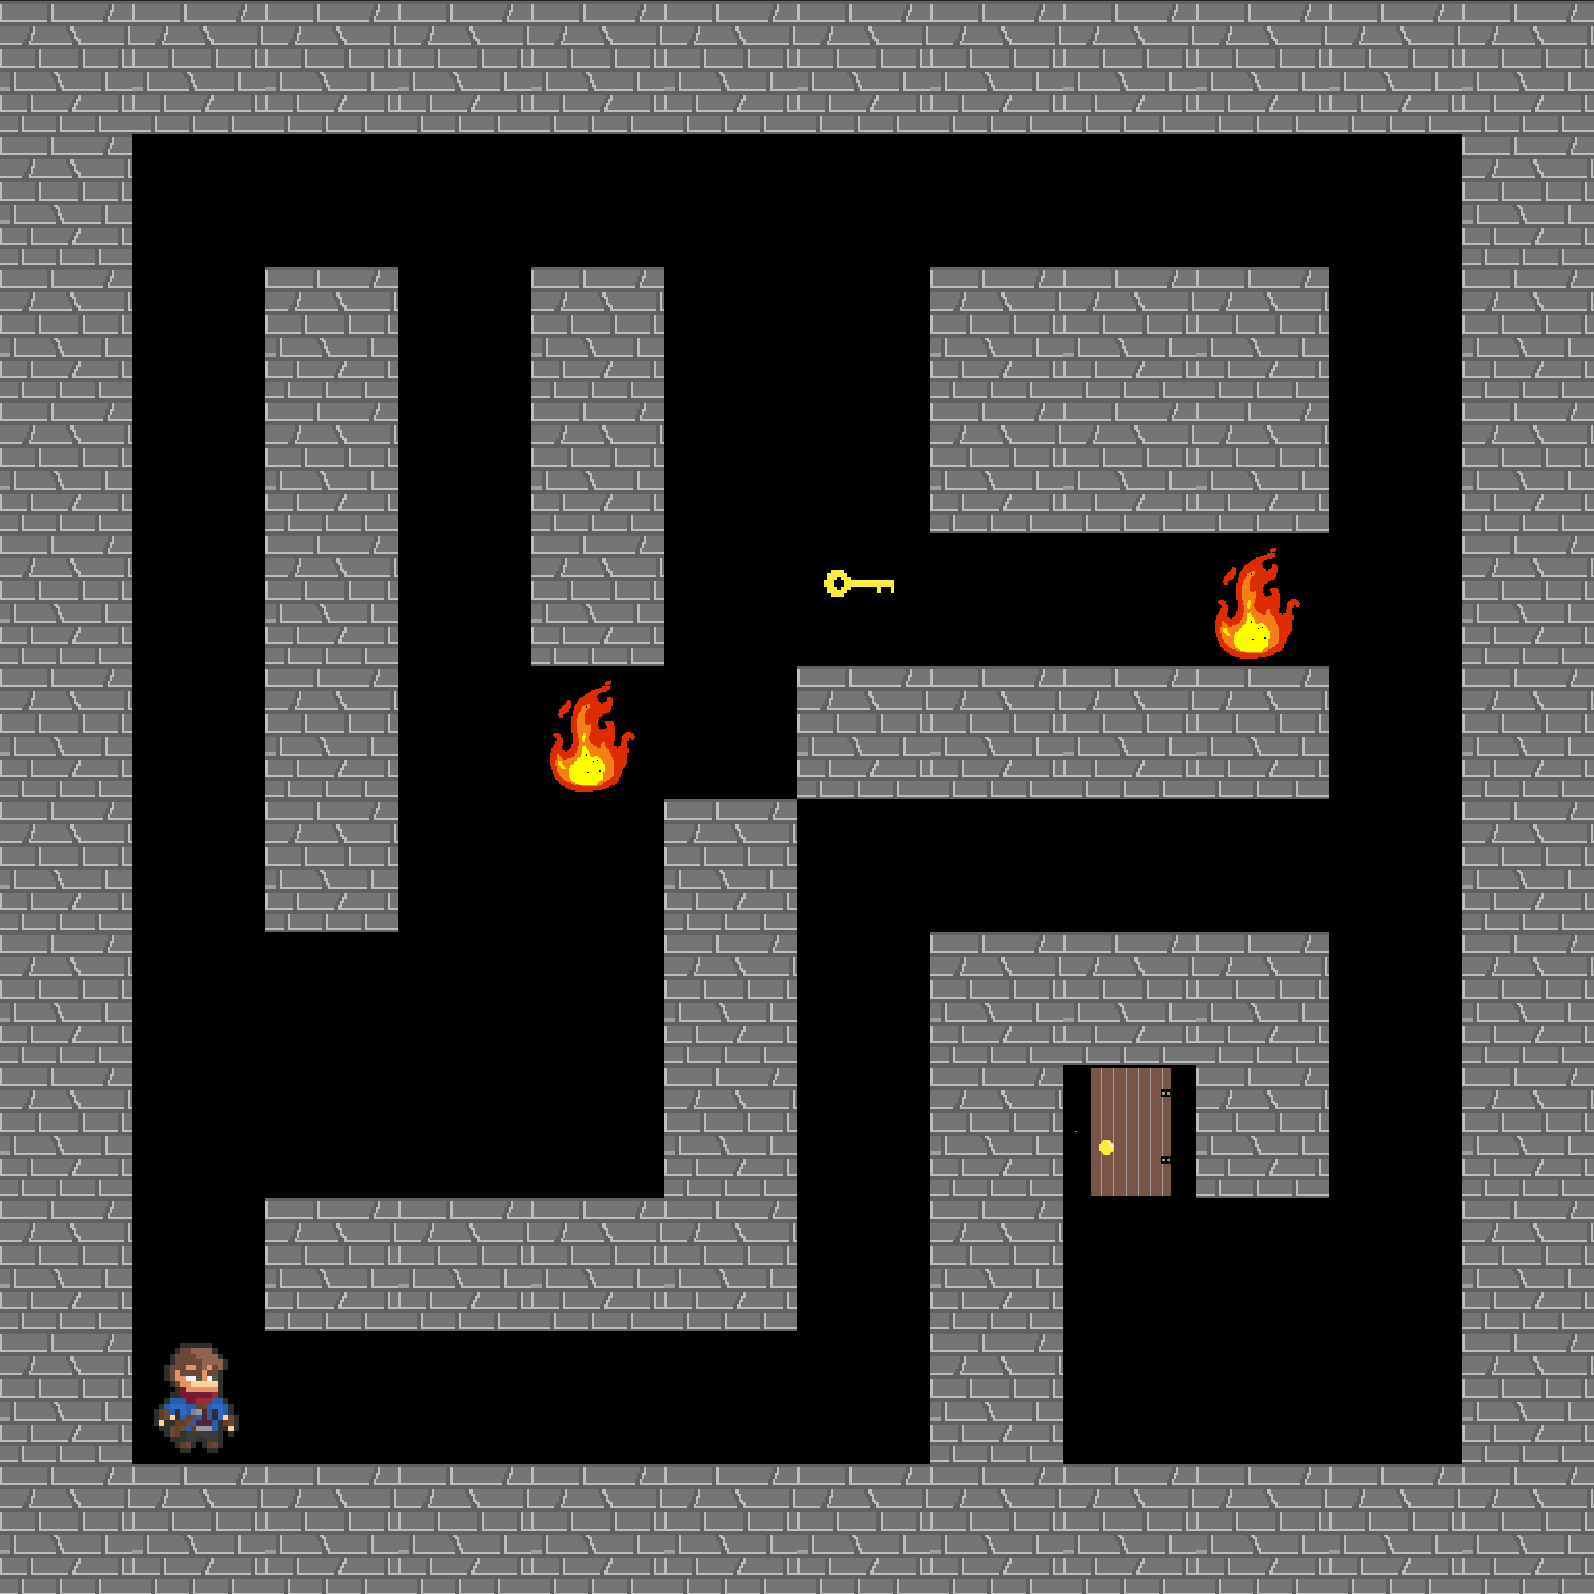
\includegraphics[width=0.5\columnwidth]{q6.png}
    \caption{}
    \label{fig:q6}
\end{figure}

This environment can be modelled as an MDP: the states correspond to the adventurer's $(x,y)$ position in the maze and whether he currently possesses the key. Rewards are 0 on every time step the agent has not reached the end with the key, 1 for successfully completing the maze, and -100 if the agent touches fire. The agent would like to finish the maze as quickly as possible, so all rewards have a discount rate $\gamma = 0.95$.

Your task is to use your knowledge of reinforcement learning to help the agent solve the maze as quickly as possible. Specifically, you will implement the Q-learning algorithm. Blueprint code is provided in the \textbf{q6} directory. An implementation of the environment and main training loop are already provided, you only need to implement the functions in \textbf{agent.py}. We also provide an implementation of an action-value table in \textbf{action\_value\_table.py}. The agent will use a epsilon-greedy behaviour policy to ensure adequate exploration of the maze. The constants $\gamma$, $\epsilon$ and step size are already given as attributes of the agent, please use these in your implementation. 

All external python libraries required are in requirements.txt, use the command \textbf{pip3 install -r requirements.txt} to install them. In this assignment you will need to sample from probability distributions. Please use \textbf{numpy.random.rand()} (\url{https://numpy.org/doc/stable/reference/random/generated/numpy.random.rand.html}) to generate a  floating point number uniformly at random and \textbf{numpy.random.choice()} (\url{https://numpy.org/doc/stable/reference/random/generated/numpy.random.choice.html}) to uniformly randomly select an element from a list.  

We have provided public test cases for this assignment; run them using \textbf{python3 tests.py}.
(These tests take approximately 4 minutes to run on my laptop.)

We will test your program by running (a copy of) the module defined in \textbf{main.py}.  You can run the same program using \textbf{python3 main.py}.  An automated graphic will display a final episode after training has been completed, and a learning curve, showing the length of episodes over time will be generated in \textbf{learning\_curve.png}. 

\begin{enumerate}
    \item \points{3}
    In the function \textbf{display\_final\_episode()} the agent is evaluated using a \textit{greedy} policy, instead of an $\epsilon$-greedy policy.  Why does it make sense to evaluate the agent this way? Would this still work with Sarsa?
    \begin{answer}{1.5in}
    % Put your answer here
    \end{answer}

    \item \points{3}
    Could Monte Carlo control be used instead to solve this problem? Justify your answer.
    \begin{answer}{1.5in}
    % Put your answer here
    \end{answer}
        
    
\end{enumerate}





\end{enumerate}

%------------------------------------------------------------------------------------------
\section*{Submission}
The assignment you downloaded from eClass is a single ZIP archive which includes this document as a PDF {\em and} its \LaTeX{} source as well as code.

\medskip

Each assignment is to be submitted electronically via eClass by the due date.
\textbf{Your submission must be a zip containing your answers and code. Please name your zip file with your CCID. } This zip should contain your PDF with answers and the \texttt{q6/} subdirectory containing your code.
Please do not change the structure of \texttt{q6/} subdirectory within your submission. 

To generate the PDF file with your answers you can do any of the following:

\begin{itemize}
    \item
    insert your answers into the provided \LaTeX{} source file between \verb|\begin{answer}| and \verb|\end{answer}|. Then run the source through \LaTeX{} to produce a PDF file;

    \item print out the provided PDF file and legibly write your answers in the blank spaces under each question. Make sure you write as legibly as possible for we cannot give you any points if we cannot read your hand-writing. Then scan the pages and include the scan in your ZIP submission to be uploaded on eClass;

    \item use your favourite text processor and type up your answers there. Make sure you number your answers in the same way as the questions are numbered in this assignment.
\end{itemize}




%\bibliography{gtdt}
%\bibliographystyle{apalike}
\end{document}
